\documentclass[10pt]{article}

  \usepackage{pgfplots}
\pgfplotsset{compat=newest}
%% the following commands are needed for some matlab2tikz features
\usetikzlibrary{plotmarks}
\usetikzlibrary{arrows.meta}
\usepgfplotslibrary{patchplots}
\usepackage{grffile}
\usepackage{amsmath}


%\usepackage{fullpage}
\usepackage[top=1in, bottom=1in, left=0.8in, right=1in]{geometry}
\usepackage{multicol}
%\usepackage{wrapfig}
%\usepackage{listings}
\usepackage{caption}
\usepackage{subcaption}
\usepackage{hyperref}
\usepackage{xcolor}
%\usepackage{soul}
\usepackage{graphicx}
\usepackage[pdf]{pstricks}

\definecolor{lightblue}{rgb}{.80,.9,1}
\newcommand{\hl}[1]
    {\par\colorbox{lightblue}{\parbox{\linewidth}{#1}}}

\newcommand{\defn}{\stackrel{\textrm{\scriptsize def}}{=}}

\setlength{\columnsep}{0.1pc}

\title{Numerical Study of The Generalised Serre-Green-Naghdi Model}
%\author{Christopher Zoppou -- \texttt{christopher.zoppou@anu.edu.au}, Dimitrios Mitsotakis -- \texttt{dmitsot@gmail.com}, Stephen Roberts -- \texttt{stephen.roberts@anu.edu.au}, Jordan Pitt}

% TIME ON EVERY PAGE AS WELL AS THE FILE NAME
\usepackage{fancyhdr}
\usepackage{currfile}
\usepackage[us,12hr]{datetime} % `us' makes \today behave as usual in TeX/LaTeX
\fancypagestyle{plain}{
\fancyhf{}
\rfoot{\emph{\footnotesize \textcopyright  Serre Notes by C. Zoppou, D. Mitsatakis and S. Roberts.}
 \\ File Name: {\currfilename} \\ Date: {\ddmmyyyydate\today} at \currenttime}
\lfoot{Page \thepage}
\renewcommand{\headrulewidth}{0pt}}
\pagestyle{plain}

\definecolor{mycolor1}{rgb}{0.00000,0.44700,0.74100}%
\definecolor{mycolor2}{rgb}{0.85000,0.32500,0.09800}%
\definecolor{mycolor3}{rgb}{0.92900,0.69400,0.12500}%
\definecolor{mycolor4}{rgb}{0.49400,0.18400,0.55600}%
\definecolor{mycolor5}{rgb}{0.46600,0.67400,0.18800}%
\definecolor{mycolor6}{rgb}{0.30100,0.74500,0.93300}%

\newcommand\T{\rule{0pt}{5ex }}       % Top table strut
\newcommand\B{\rule[-4ex]{0pt}{4ex }} % Bottom table strut

\newcommand\TM{\rule{0pt}{2.8ex }}       % Top matrix strut
\newcommand\BM{\rule[-2ex]{0pt}{2ex }} % Bottom matrix strut

\newcommand\solidrule[1][0.25cm]{\rule[0.5ex]{#1}{1.5pt}}
\newcommand\dashedrule{\mbox{%
		\solidrule[2mm]\hspace{2mm}\solidrule[2mm]}}

\begin{document}

\maketitle

\vspace{-0.3in}
\noindent
\rule{\linewidth}{0.4pt}

\tableofcontents

%-------------------------------------------------
\section{Introduction}
%-------------------------------------------------



%-------------------------------------------------
\section{Generalised Serre-Green-Naghdi Equations}
%-------------------------------------------------
Clamond and Dutykh\cite{Clamond-Dutykh-2018-237} derived the generalised Serre-Green-Naghdi (gSGN) equations:

\begin{subequations}
	\begin{gather}
	\dfrac{\partial h}{\partial t} + \dfrac{\partial (uh)}{\partial x} = 0
	\label{eq:gSGNh}
	\end{gather}
	\begin{gather}
	\dfrac{\partial (uh)}{\partial t} + \dfrac{\partial }{\partial x} \left( u^2h + \dfrac{gh^2}{2} + \frac{1}{3} h^2 \Gamma \right)= 0
	\label{eq:gSGNuh}
	\end{gather}
	\begin{multline}
	\dfrac{\partial}{\partial t}\left[\frac{1}{2}hu^2 + \dfrac{1}{4}\left(\frac{2}{3} + \beta_1\right) h^3 \dfrac{\partial u}{\partial x}\dfrac{\partial u}{\partial x} + \frac{1}{2}gh^2\left(1 + \frac{1}{2}\beta_2 \dfrac{\partial h}{\partial x} \dfrac{\partial h}{\partial x}\right) \right] \\
	\dfrac{\partial}{\partial x}\left[uh\left(\frac{1}{2}u^2 + \dfrac{1}{4}\left(\frac{2}{3} + \beta_1\right)h^2\dfrac{\partial u}{\partial x}\dfrac{\partial u}{\partial x} + gh\left(1 + \frac{1}{4}\beta_2\dfrac{\partial h}{\partial x}\dfrac{\partial h}{\partial x} \right)   + \frac{1}{3} h\Gamma  \right) + \frac{1}{2}\beta_2 g h^3\dfrac{\partial h}{\partial x}\dfrac{\partial u}{\partial x} \right]
	=0
	\label{eq:gSGNE}
	\end{multline}
	where
	\begin{equation}
	\Gamma = \frac{3}{2}\left(\frac{2}{3} + \beta_1\right)h \left[\frac{\partial u}{\partial x}\frac{\partial u}{\partial x} - \frac{\partial^2 u}{\partial x \partial t} - u\frac{\partial^2 u}{\partial x^2}\right] - \frac{3}{2} \beta_2 g\left[h \frac{\partial^2 h}{\partial x^2} + \frac{1}{2} \frac{\partial h}{\partial x}\frac{\partial h}{\partial x} \right]
	\end{equation}
	\label{eq:gSGN}
\end{subequations}

These equations have the same order of approximation in the lagrangian density (dispersion properties?) when $\beta_1 = \beta_2$. The interesting thing about the equations though, is that we will conserve mass, momentum and energy for all values of $\beta_j$. 

From these equations the SWWE, the Serre equations and the regularised SWWE \cite{Clamond-Dutykh-2018-237} can be recovered for certain values of $\beta_1$ and $\beta_2$. 

%\begin{itemize}
%	\item When $\beta_1 = 2\epsilon -\frac{2}{3}$ and $\beta_2 = 2 \epsilon$ we get the regularised Saint Venant equations of \cite{Clamond-Dutykh-2018-237}. Which admit the SWWE when $\epsilon = 0$. 
%	\item When $\beta_1 = \beta_2$ we get the improved Serre-Green-Naghdi equations, which when $\beta_1 =\beta_2 = 0$ are the Serre-Green-Naghdi equations. 
%\end{itemize}

\begin{table}
	\centering
	\begin{tabular}{c | c | c}
		Resulting Equations &$\beta_1$ & $\beta_2$  \\
		\hline 
		Serre Equations & $0$ & $0$ \\
		SWWE Equations & $-\dfrac{2}{3}$ & $0$ \\
		Regularised SWWE Equation Family & free variable & $\beta_1 + \dfrac{2}{3}$  \\
		Modified Dispersion Serre Equation Family & free variable & $\beta_1$
	\end{tabular}
	\caption{Showing various combinations of $\beta$ values and equivalent equations}
\end{table}

%-------------------------------------------------
\subsection{Alternative Conservative Form of the gSGN}
%-------------------------------------------------

A major difficulty with solving the SGN is that the dispersive terms contain a mixed spatial-temporal derivative term which is difficult to handle numerically. This mixed derivative term can be rewritten  so that the Serre equations can be expressed in conservation law form, with the water depth and a new quantity as conservative variables. This reformulation allows standard techniques for solving conservation laws to be applied to the Serre equations, even though the Serre equations are neither hyperbolic nor parabolic.

Consider the Serre equations written for a horizontal bed. The flux term in the momentum equation, \eqref{eq:gSGNuh} contains a mixed spatial and temporal derivative term which is difficult to treat numerically. It is possible to replace this term  by a combination of spatial and temporal derivative terms by making the following observation
\begin{multline}
\dfrac{\partial^2}{\partial x \partial t} \left ( \frac{1}{3}\left(1 + \frac{3}{2} \beta_1\right) h^3 \dfrac{\partial u}{\partial x} \right ) =   \frac{1}{3}\left(1 + \frac{3}{2} \beta_1\right) \dfrac{\partial }{\partial t} \left ( 3h^2 \dfrac{\partial h}{\partial x} \dfrac{\partial u}{\partial x} + h^3 \dfrac{\partial^2 u}{\partial x^2} \right ) \\=  \frac{1}{3}\left(1 + \frac{3}{2} \beta_1\right)
\dfrac{\partial }{\partial x} \left ( 3 h^2 \dfrac{\partial h}{\partial t} \dfrac{\partial u}{\partial x} + h^3 \dfrac{\partial^2 u}{\partial x \partial t} \right ).
\end{multline}
Rearranging and making use of the continuity equation, \eqref{eq:gSGNh} the momentum equation, \eqref{eq:gSGNuh} becomes
\begin{multline}
\dfrac{\partial }{\partial t} \left ( u h -  \frac{1}{3}\left(1 + \frac{3}{2} \beta_1\right) \dfrac{\partial}{\partial x} \left [h^3 \dfrac{\partial u}{\partial x}  \right ] \right ) \\ + \dfrac{\partial}{\partial x} \left ( u\left[uh - \frac{1}{3}\left(1 + \frac{3}{2} \beta_1\right) \dfrac{\partial }{\partial x} \left [ h^3 \dfrac{\partial u}{\partial x} \right ]\right] + \dfrac{gh^2}{2} - \frac{2}{3}\left(1 + \frac{3}{2} \beta_1\right) h^3\dfrac{\partial u}{\partial x}\dfrac{\partial u}{\partial x}  - \frac{1}{2} \beta_2 g h^2 \left[h\frac{\partial^2 h}{\partial x^2} + \frac{1}{2}\frac{\partial h}{\partial x}\frac{\partial h}{\partial x}\right]\right ) = 0.
\end{multline}
The momentum equation can be written in conservation law form as
\begin{gather}\label{eq:G_momentum}
\dfrac{\partial G }{\partial t}  + \dfrac{\partial}{\partial x} \left ( uG + \dfrac{gh^2}{2} - \frac{2}{3}\left(1 + \frac{3}{2} \beta_1\right) h^3\dfrac{\partial u}{\partial x}\dfrac{\partial u}{\partial x}  - \frac{1}{2} \beta_2 g h^2  \left[h\frac{\partial^2 h}{\partial x^2} + \frac{1}{2}\frac{\partial h}{\partial x}\frac{\partial h}{\partial x}\right]\right ) = 0.
\end{gather}
where a new conserved quantity, $G$ is given by
\begin{gather*}
G = uh - \frac{1}{3}\left(1 + \frac{3}{2} \beta_1\right) \dfrac{\partial }{\partial x} \left ( h^3 \dfrac{\partial u}{\partial x} \right ).
\end{gather*}
This expands the conserved variable introduced by \cite{Clamond-Dutykh-2018-237}, as well as in the Serre equations []. 

Thus we have the following conservation equations

\begin{subequations}
\begin{gather}
\dfrac{\partial h}{\partial t} + \dfrac{\partial (uh)}{\partial x} = 0
\label{eq:gSGN_Gh}
\end{gather}
\begin{gather}
\dfrac{\partial G }{\partial t}  + \dfrac{\partial}{\partial x} \left ( uG + \dfrac{gh^2}{2} - \frac{2}{3}\left(1 + \frac{3}{2} \beta_1\right) h^3\dfrac{\partial u}{\partial x}\dfrac{\partial u}{\partial x}  - \frac{1}{2} \beta_2 g h^2  \left[h\frac{\partial^2 h}{\partial x^2} + \frac{1}{2}\frac{\partial h}{\partial x}\frac{\partial h}{\partial x}\right]\right ) = 0.
\label{eq:gSGN_GG}
\end{gather}
with
\begin{gather}\label{eq:G_divergent}
G = uh - \frac{1}{3}\left(1 + \frac{3}{2} \beta_1\right) \dfrac{\partial }{\partial x} \left ( h^3 \dfrac{\partial u}{\partial x} \right ).
\end{gather}
\end{subequations}

\subsection{Dispersion Relation of Linearised gSGN}

Assuming that
\begin{align*}
h(x,t) &= h_0 + \delta \eta(x,t) + O(\delta^2)\\
u(x,t) &= u_0 + \delta v(x,t) + O(\delta^2)
\end{align*}

By substituting these forms into the linearised Serre equations and neglecting $O(\delta^2)$ terms, we get the linearised regularised Serre equations. We also substitute $\eta_t$ using the mass equation into the momentum equation. 


\begin{subequations}
	\begin{equation}
	\label{eqlinhd}
	(\delta\eta)_t + u_0 (\delta \eta)_x + h_0 (\delta v)_x = 0
	\end{equation}
	\begin{equation}
	\label{eqlinuhd}
	h_0(\delta v)_t + gh_0(\delta \eta)_x + h_0u_0 (\delta v)_x - \frac{1}{3}\left(1 + \frac{3}{2}\beta_1\right) h_0^3(\delta v)_{xxt} - \frac{1}{3}\left(1 + \frac{3}{2}\beta_1\right) h_0^3 u_0 (\delta v)_{xxx} -\frac{g\beta_2}{2}h_0^3 (\delta \eta)_{xxx}  = 0
	\end{equation}
\end{subequations}

We can remove the $\delta$ term, either by removing the common factor, or absorbing it into $\eta$ and $v$ to get

\begin{subequations}
	\begin{equation}
	\label{eqlinh}
	\eta_t + u_0 \eta_x + h_0 v_x = 0
	\end{equation}
	\begin{equation}
	\label{eqlinuh}
	h_0(v)_t + gh_0(\eta)_x + h_0u_0 (v)_x - \frac{1}{3}\left(1 + \frac{3}{2}\beta_1\right) h_0^3(v)_{xxt} - \frac{1}{3}\left(1 + \frac{3}{2}\beta_1\right) h_0^3 u_0 ( v)_{xxx} -\frac{g\beta_2}{2}h_0^3 (\eta)_{xxx}  = 0
	\end{equation}
\end{subequations}

We now assume that $\eta(x,t) = H \exp\left(i (k x - \omega t)\right)$,  $v(x,t) = U \exp\left(i (k x - \omega t)\right)$
\begin{align*}
\eta(x,t) &= H \exp\left(i (k x - \omega t)\right) \\
v(x,t) &= U \exp\left(i (k x - \omega t)\right)
\end{align*}

substituting these into the linearised Serre equation we get

\begin{subequations}
	\begin{equation}
	\label{eqlinhexp}
	\left[H u_0 k - H \omega + U h_0k\right]i \exp\left[i \left(k x - \omega t\right)\right] = 0
	\end{equation}
	\begin{multline}
	\label{eqlinuhexp}
	\bigg[3H \beta_2 g h_0^2 k^3 + 6Hgk - 3U \beta_1 \omega h_0^2 k^2 + 3U\beta_1 h_0^2 k^3 u_0\\ - 2U \omega h_0^2 k^2 - 6U \omega + 2U h_0^2 k^3 u_0 + 6U k u_0\bigg] i \frac{h_0}{6} \exp\left[i \left(k x - \omega t\right)\right] = 0
	\end{multline}
\end{subequations}


This can be written as
\begin{equation}
\begin{bmatrix}
u_0k - \omega & h_0 k \\
3 \beta_2 h_0^2 k^3 + 6k g & -3 \beta_1 \omega h_0^2 k^2 + 3 \beta_1 h_0^2 k^3 u_0 - 2\omega h_0^2 k^2 - 6\omega + 2h_0^2 k^3 u_0 + 6ku_0
\end{bmatrix}
\begin{bmatrix}
H \\ U
\end{bmatrix} = 0
\end{equation}

Which has non-trivial solutions when the determinant is zero. 

The determinant of this matrix is
\begin{equation}
\left(3\beta_1 h_0^2 k^2 + 2h_0^2 k^2 + 6\right)\omega^2 - 2 u_0k \left(3\beta_1 h_0^2 k^2 + 2h_0^2 k^2 + 6\right)\omega  + u_0^2 k^2 \left(3\beta_1 h_0^2 k^2 + 2h_0^2 k^2 + 6\right) - g h_0 k^2 \left(3 \beta_2 h_0^2 k^2 + 6\right)
\end{equation} 

To get non-trivial solution we have

\begin{equation}
\left(3\beta_1 h_0^2 k^2 + 2h_0^2 k^2 + 6\right)\omega^2 - 2 u_0k \left(3\beta_1 h_0^2 k^2 + 2h_0^2 k^2 + 6\right)\omega  + u_0^2 k^2 \left(3\beta_1 h_0^2 k^2 + 2h_0^2 k^2 + 6\right) - g h_0 k^2 \left(3 \beta_2 h_0^2 k^2 + 6\right) = 0
\end{equation} 

\begin{equation}
\omega^2 - 2 u_0k \omega  + u_0^2 k^2 - g h_0 k^2 \dfrac{3 \beta_2 h_0^2 k^2 + 6}{\left(3\beta_1 h_0^2 k^2 + 2h_0^2 k^2 + 6\right)} 
\end{equation} 

Using quadratic equation, or another quadratic polynomial solver we get that

\begin{equation}
\omega^\pm = u_0 k \pm k \sqrt{gh_0} \sqrt{\dfrac{3 \beta_2 h_0^2 k^2 + 6}{\left(3\beta_1 h_0^2 k^2 + 2h_0^2 k^2 + 6\right)} }
\end{equation}

\begin{equation}
\omega^\pm = u_0 k \pm k \sqrt{gh_0} \sqrt{\dfrac{\beta_2 h_0^2 k^2 + 2}{\left(\frac{2}{3} + \beta_1\right) h_0^2 k^2 + 2} }
\end{equation}


Thus we have the following regimes
\begin{itemize}
	\item SWWE wavespeeds (non-dispersive): occurs when $\beta_2 = \frac{2}{3} + \beta_1$ then $\omega^\pm = k\left(u_0\pm \sqrt{gh_0}\right)$ (\cite{Clamond-Dutykh-2018-237}).
	\item Serre wavespeeds - when $\beta_1 = \beta_2 = 0$ - we get $\omega^\pm = k\left(u_0\pm \sqrt{gh_0} \sqrt{\dfrac{3}{3 + h_0^2 k^2}}\right)$
	\item For other values of $\beta_1$ and $\beta_2$ we can vary the wavespeeds, in certain situations this will lead to a better approximation of the linear wavespeed of waves than the Serre equations ( \cite{Clamond-Dutykh-2018-237}), in others it will be worse. We show an example below.
\end{itemize}

Now for the group speed
\begin{equation}
v^\pm_g = \frac{\partial \omega^\pm }{\partial k}= u_0  \pm  \sqrt{gh_0} \sqrt{\dfrac{\beta_2 h_0^2 k^2 + 2}{\left( \left(\frac{2}{3} + \beta_1\right) h_0^2 k^2 + 2\right)} } \pm \dfrac{k\sqrt{gh_0}}{\beta_2 h_0^2 k^2 +2} \left[\sqrt{\dfrac{\beta_2 h_0^2 k^2 + 2}{\left( \left(\frac{2}{3} + \beta_1\right) h_0^2 k^2 + 2\right)} } \left( \beta_2 h_0^2 k - \dfrac{h_0^2 k \left(\beta_1 + \frac{2}{3}\right)\left(\beta_2h_0^2k^2 + 2\right)}{h_0^2 k^2 \left(\beta_1 + \frac{2}{3}\right) + 2} \right)\right]
\end{equation} 

\begin{multline*}
= u_0  \pm  \sqrt{gh_0} \sqrt{\dfrac{\beta_2 h_0^2 k^2 + 2}{\left( \left(\frac{2}{3} + \beta_1\right) h_0^2 k^2 + 2\right)} } \pm \\ \dfrac{k\sqrt{gh_0}}{\beta_2 h_0^2 k^2 +2} \left[\sqrt{\dfrac{\beta_2 h_0^2 k^2 + 2}{\left( \left(\frac{2}{3} + \beta_1\right) h_0^2 k^2 + 2\right)} } \left(  \dfrac{\beta_2 h_0^2 k^2 \left[h_0^2 k^2 \left(\beta_1 + \frac{2}{3}\right) + 2\right] -h_0^2 k \left(\beta_1 + \frac{2}{3}\right)\left(\beta_2h_0^2k^2 + 2\right)}{h_0^2 k^2 \left(\beta_1 + \frac{2}{3}\right) + 2} \right)\right]
\end{multline*} 

\begin{multline*}
= u_0  \pm  \sqrt{gh_0} \sqrt{\dfrac{\beta_2 h_0^2 k^2 + 2}{\left( \left(\frac{2}{3} + \beta_1\right) h_0^2 k^2 + 2\right)} } \pm \\ \dfrac{k\sqrt{gh_0}}{\beta_2 h_0^2 k^2 +2} \left[\sqrt{\dfrac{\beta_2 h_0^2 k^2 + 2}{\left( \left(\frac{2}{3} + \beta_1\right) h_0^2 k^2 + 2\right)} } \left(  \dfrac{  \beta_2 h_0^4 k^3 \left(\beta_1 + \frac{2}{3}\right)  + 2\beta_2 h_0^2 k -h_0^2 k \left(\beta_1 + \frac{2}{3}\right)\left(\beta_2h_0^2k^2 + 2\right)}{h_0^2 k^2 \left(\beta_1 + \frac{2}{3}\right) + 2} \right)\right]
\end{multline*} 

\begin{multline*}
= u_0  \pm  \sqrt{gh_0} \sqrt{\dfrac{\beta_2 h_0^2 k^2 + 2}{\left( \left(\frac{2}{3} + \beta_1\right) h_0^2 k^2 + 2\right)} } \pm \\ \dfrac{k\sqrt{gh_0}}{\beta_2 h_0^2 k^2 +2} \left[\sqrt{\dfrac{\beta_2 h_0^2 k^2 + 2}{\left( \left(\frac{2}{3} + \beta_1\right) h_0^2 k^2 + 2\right)} } \left(  \dfrac{  \beta_2 h_0^4 k^3 \left(\beta_1 + \frac{2}{3}\right)  + 2\beta_2 h_0^2 k -  \beta_2\left(\beta_1 + \frac{2}{3}\right)h_0^4k^3 -    2 h_0^2 k \left(\beta_1 + \frac{2}{3}\right)}{h_0^2 k^2 \left(\beta_1 + \frac{2}{3}\right) + 2} \right)\right]
\end{multline*} 


\begin{multline*}
= u_0  \pm  \sqrt{gh_0} \sqrt{\dfrac{\beta_2 h_0^2 k^2 + 2}{\left( \left(\frac{2}{3} + \beta_1\right) h_0^2 k^2 + 2\right)} } \pm \\ \dfrac{k\sqrt{gh_0}}{\beta_2 h_0^2 k^2 +2} \left[\sqrt{\dfrac{\beta_2 h_0^2 k^2 + 2}{\left( \left(\frac{2}{3} + \beta_1\right) h_0^2 k^2 + 2\right)} } \left(  \dfrac{  2\beta_2 h_0^2 k  -    2 h_0^2 k \left(\beta_1 + \frac{2}{3}\right)}{h_0^2 k^2 \left(\beta_1 + \frac{2}{3}\right) + 2} \right)\right]
\end{multline*} 

\begin{multline*}
= u_0  \pm  \sqrt{gh_0} \sqrt{\dfrac{\beta_2 h_0^2 k^2 + 2}{\left( \left(\frac{2}{3} + \beta_1\right) h_0^2 k^2 + 2\right)} } \pm  2\dfrac{k^2h_0^2\sqrt{gh_0}}{\beta_2 h_0^2 k^2 +2} \left[\sqrt{\dfrac{\beta_2 h_0^2 k^2 + 2}{\left( \left(\frac{2}{3} + \beta_1\right) h_0^2 k^2 + 2\right)} } \left(  \dfrac{\beta_2  -    \beta_1 - \frac{2}{3}}{h_0^2 k^2 \left(\beta_1 + \frac{2}{3}\right) + 2} \right)\right]
\end{multline*} 

\begin{equation*}
= u_0  \pm  \sqrt{gh_0} \sqrt{\dfrac{\beta_2 h_0^2 k^2 + 2}{\left( \left(\frac{2}{3} + \beta_1\right) h_0^2 k^2 + 2\right)} } \left[1 +  \dfrac{\beta_2 - \beta_1 - \frac{2}{3}}{\left(\frac{1}{2}\beta_2 h_0^2 k^2 +1\right)\left( \left(\frac{1}{3} + \beta_1\right) h_0^2 k^2 + 1\right)}\right] 
\end{equation*} 


When $\beta_2 = \frac{2}{3} + \beta_1$ then the group speed is equal to the phase speed of the Shallow Water Wave equations. When $\beta_2 = \beta_1 = 0$ then we get

\begin{equation*}
= u_0  \pm  \sqrt{gh_0} \sqrt{\dfrac{2}{\left( \frac{2}{3} h_0^2 k^2 + 2\right)} } \left[1 + \dfrac{- \frac{1}{3}}{\left( \frac{1}{3} h_0^2 k^2 + 1\right)}\right] 
\end{equation*} 

\begin{equation*}
= u_0  \pm  \sqrt{gh_0} \sqrt{\dfrac{3}{  h_0^2 k^2 + 3} } \left[1 -  \dfrac{1}{ h_0^2 k^2 + 3}\right] 
\end{equation*} 

which matches [Zoppo,pitt,paper on FDVM methods for Serre equations / Chris thesis]


\subsubsection{Wave Speed Bounds}

First we want to show that phase and group speed are bounded, when treated as functions of $k$.
The phase speed is:
\begin{equation}
v^\pm_p = \frac{\omega^\pm}{k}=u_0 \pm  \sqrt{gh_0} \sqrt{\dfrac{\beta_2 h_0^2 k^2 + 2}{\left( \left(\frac{2}{3} + \beta_1\right) h_0^2 k^2 + 2\right)} }
\end{equation} 

For $\beta_1 \ge -\frac{2}{3}$ and $\beta_2 \ge 0$ we have that 

\begin{equation}
\dfrac{\beta_2 h_0^2 k^2 + 2}{\left( \left(\frac{2}{3} + \beta_1\right) h_0^2 k^2 + 2\right)}
\end{equation}

is a montone function in terms of $h_0k$, it is monotone decreasing if $\beta_2 \le \frac{2}{3} + \beta_1$ and monotone increasing if $\beta_2 \ge \frac{2}{3} + \beta_1$.
 
We have the following limits

as $k \rightarrow 0$
\begin{equation}
 v^\pm_p = u_0 \pm \sqrt{gh_0}
\end{equation} 

as $k \rightarrow \infty$
\begin{equation}
v^\pm_p = u_0 \pm \sqrt{gh_0} \sqrt{\dfrac{\beta_2}{\frac{2}{3} + \beta_1}}
\end{equation}

When $\dfrac{\beta_2}{\frac{2}{3} + \beta_1} \le 1$ we have

\begin{equation}
u_0 -  \sqrt{gh_0} \le  v^-_p \le u_0 - \sqrt{gh_0} \sqrt{\dfrac{\beta_2}{\frac{2}{3} + \beta_1}} \le u_0 \le u_0 + \sqrt{gh_0} \sqrt{\dfrac{\beta_2}{\frac{2}{3} + \beta_1}} \le   v^+_p  \le u_0 +   \sqrt{gh_0}
\end{equation}

(includes Serre and regularised SWWE). For Serre the $k \rightarrow \infty $ bounds are $u_0$, so inequality simplifies for regularised SWWE, phase speed is fixed as $k$ changes. 

when $\dfrac{\beta_2}{\frac{2}{3} + \beta_1} > 1$ we have

\begin{equation}
u_0 - \sqrt{gh_0} \sqrt{\dfrac{\beta_2}{\frac{2}{3} + \beta_1}} \le v^-_p \le u_0 -  \sqrt{gh_0} \le  u_0 \le u_0 + \sqrt{gh_0} \le   v^+_p  \le u_0 +  \sqrt{gh_0} \sqrt{\dfrac{\beta_2}{\frac{2}{3} + \beta_1}}
\end{equation}

Region $1$ is what we expect, dispersive waves travel behind the shock front, Region $2$ is inverted and we begin to see dispersive waves travel in front of the shock. 

%Region Plot
%\beta_2 = -2/3 + beta_1

We thus have the following plots

\begin{figure}
		\centering
		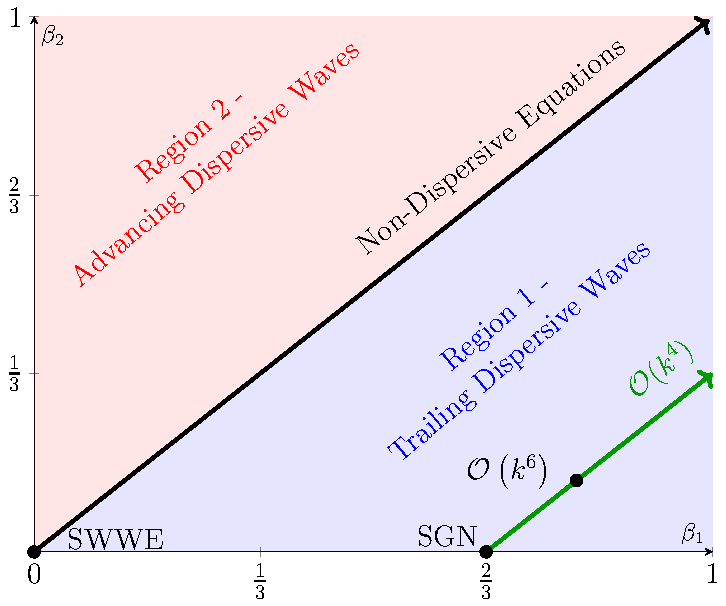
\includegraphics[width=0.4\textwidth]{./Figures/Explanation/BetaPlotAll.pdf}
	\caption{Wave speed region plots showing important families of equations and particular members of these families.}
\end{figure}


\section{Numerical Method}


\section{Validation}

\subsection{Analytic Solutions}
\subsubsection{Serre Equations ($\beta_1=\beta_2 =0$) - Solitary Travelling Wave Solution}
When $\beta_1 = \beta_2 = 0$ the gSGN are equivalent to the SGN equations which admit the following travelling wave solution

\begin{subequations}
	\begin{equation}
	h(x,t) = a_0 + a_1 \text{sech}^2\left( \kappa (x - ct) \right)
	\end{equation}
	\begin{equation}
	u(x,t) = c \left( 1- \dfrac{a_0}{h(x,t)} \right)
	\end{equation}
	where
	\begin{equation}
	\kappa = \dfrac{\sqrt{3a_1}}{2a_0 \sqrt{a_0 + a_1}}
	\end{equation}
	\begin{equation}
	c = \sqrt{g\left(a_0 + a_1\right)}
	\end{equation}
\end{subequations}


%% RESULTS %%

Results - Example,Convergence and Conservation Plot

\subsubsection{SWWE ( $\beta_1= -\frac{2}{3}$ and $ \beta_2 =0$ ) - Dambreak Solution }
\begin{align}
h(x,0) & = \left\lbrace \begin{array}{c c}
h_0 & x < 0\\
h_1 & x \ge 0
\end{array} \right.  \\
u(x,0) &= 0 \\
G(x,0) &= 0
\end{align}

We have an analytic solution for the SWWE for the discontinuous limit of these equations as $\alpha \rightarrow 0$. It is 3 constant states $(h_0,0)$, $(h_s,u_s)$ and $(h_1,0)$ where
\begin{equation}
h_s = \dfrac{h_0}{2}  \sqrt{1 + 8 \left( \dfrac{2 h_s}{h_s - h_0} \left(\dfrac{\sqrt{gh_1} - \sqrt{gh_s}}{\sqrt{gh_0}}\right)\right)^2 - 1}
\end{equation}
\begin{equation}
u_s = 2\left(\sqrt{gh_1} - \sqrt{gh_s} \right).
\end{equation}
Where $(h_0,0)$ and $(h_s,u_s)$ are joined by a 


Results - Example and Conservation Table


\subsection{Forced Solutions}
To demonstate the validity and versatility of our method to solve the gSGN whilst allowing varying $\beta_i$ values, we make use of forced solutions. To generate a forced solution we consider the modified gSGN equations 

\begin{subequations}
	\begin{gather}
	\dfrac{\partial h}{\partial t} + \dfrac{\partial (uh)}{\partial x} = \dfrac{\partial h^*}{\partial t} + \dfrac{\partial (u^*h^*)}{\partial x} 
	\label{eq:gSGN_Gh_Forced}
	\end{gather}
	\begin{multline}
	\dfrac{\partial G }{\partial t}  + \dfrac{\partial}{\partial x} \left ( uG + \dfrac{gh^2}{2} - \frac{2}{3}\left(1 + \frac{3}{2} \beta_1\right) h^3\dfrac{\partial u}{\partial x}\dfrac{\partial u}{\partial x}  - \frac{1}{2} \beta_2 g h^2  \left[h\frac{\partial^2 h}{\partial x^2} + \frac{1}{2}\frac{\partial h}{\partial x}\frac{\partial h}{\partial x}\right]\right ) = \\ \dfrac{\partial G^* }{\partial t}  + \dfrac{\partial}{\partial x} \left ( u^*G^* + \dfrac{g\left(h^*\right)^2}{2} - \frac{2}{3}\left(1 + \frac{3}{2} \beta_1\right) \left(h^*\right)^3\dfrac{\partial u^*}{\partial x}\dfrac{\partial u^*}{\partial x}  - \frac{1}{2} \beta_2 g \left(h^*\right)^2  \left[h^*\frac{\partial^2 h^*}{\partial x^2} + \frac{1}{2}\frac{\partial h^*}{\partial x}\frac{\partial h^*}{\partial x}\right]\right ) 
	\label{eq:gSGN_GG_Forced}
	\end{multline}
\end{subequations}

which admit the solutions $h^*$, $u^*$ and $G^*$ assuming $G^*$ appropriately satisfies \eqref{eq:G_divergent}. Since these equations are satisfied for any chosen $h^*$, $u^*$ and $G^*$, we can generated any desired solution. Since the left hand-side of these modified equations are approximated by our numerical method, if we combine the numerical method with analytic expressions for the right handside, we have a method that approximates the forced gSGN equation with the same convergence properties as the underlying numerical method for the gSGN equations. 

Since we are free to choose $h^*$, $u^*$ and $G^*$ we can generate solutions and thus test our convergence properties for situations for which no analytic solution to the equations exist, in particular in this paper we are interested in solutions where the $\beta$ values vary in space and time. 

I have used this technique to investigate the method for the following forced solutions

\begin{subequations}
	\begin{equation}
	h^*(x,t) = a_0 + a_1 \exp\left( \dfrac{\left(x - a_2 t\right)^2}{2 a_3} \right)
	\end{equation}
	\begin{equation}
	u^*(x,t) = a_4 \exp\left( \dfrac{\left(x - a_2 t\right)^2}{2 a_3} \right)
	\end{equation}
	\begin{align}
	\beta_1(x,t) &= a_6 \\
	\beta_2(x,t) &= a_7
	\end{align}
\end{subequations}
where $G^*$ is determined by \eqref{eq:G_divergent} with the above values. 

%% RESULTS %%

Results - Example plot and L1 convergence, comment that this worked for all beta values, and we only show one for conciseness


\section{Smooth Dambreak Study}
\begin{align}
h(x,0) & = h_0 + \dfrac{h_1 - h_0}{2} \left(1 + \tanh\left(\dfrac{x}{\alpha}\right)\right)  \\
u(x,0) &= 0 \\
G(x,0) &= 0
\end{align}


\subsection{Regularised SWWE Family $\beta_2 = \frac{2}{3} + \beta_1$}
Justify interest, cite denys paper on regularised SWWE

\begin{itemize}
	\item we do get nice well behaved transitions between behaviours when varying $\beta$ values
	we get nice convergence.
	\item Although solutions look nice in h, in G there can be quite large values in the smoothed regions. However, u still looks quite nice. 
\end{itemize}

\begin{figure}
	\centering
	\begin{subfigure}{0.32\textwidth}
		\centering
		\includegraphics[width=\textwidth]{./Figures/Simulations/Study/RegSWWE/Convergence/h.pdf}
		\caption{$h$}
	\end{subfigure}
	\begin{subfigure}{0.32\textwidth}
	\centering
	\includegraphics[width=\textwidth]{./Figures/Simulations/Study/RegSWWE/Convergence/G.pdf}
	\caption{$G$}
	\end{subfigure}
	\begin{subfigure}{0.32\textwidth}
	\centering
	\includegraphics[width=\textwidth]{./Figures/Simulations/Study/RegSWWE/Convergence/u.pdf}
	\caption{$u$}
	\end{subfigure}
	\caption{Plot of example numerical solution for representative memeber of regularised SWWE family to smooth dambreak problem at $t=35s$.}
\end{figure}

\begin{figure}
	\centering
	\begin{subfigure}{0.32\textwidth}
		\centering
		\includegraphics[width=\textwidth]{./Figures/Simulations/Study/RegSWWE/Convergence/hRFtop.pdf}
		\caption{$h$ top of rarefaction fan}
	\end{subfigure}
	\begin{subfigure}{0.32\textwidth}
		\centering
		\includegraphics[width=\textwidth]{./Figures/Simulations/Study/RegSWWE/Convergence/GRFtop.pdf}
		\caption{$G$ top of rarefaction fan}
	\end{subfigure}
	\begin{subfigure}{0.32\textwidth}
		\centering
		\includegraphics[width=\textwidth]{./Figures/Simulations/Study/RegSWWE/Convergence/uRFtop.pdf}
		\caption{$u$ top of rarefaction fan}
	\end{subfigure}
	\begin{subfigure}{0.32\textwidth}
	\centering
	\includegraphics[width=\textwidth]{./Figures/Simulations/Study/RegSWWE/Convergence/hRFBot.pdf}
	\caption{$h$ bottom of rarefaction fan}
	\end{subfigure}
	\begin{subfigure}{0.32\textwidth}
	\centering
	\includegraphics[width=\textwidth]{./Figures/Simulations/Study/RegSWWE/Convergence/GRFBot.pdf}
	\caption{$G$ bottom of rarefaction fan}
	\end{subfigure}
	\begin{subfigure}{0.32\textwidth}
	\centering
	\includegraphics[width=\textwidth]{./Figures/Simulations/Study/RegSWWE/Convergence/uRFBot.pdf}
	\caption{$u$ bottom  of rarefaction fan}
	\end{subfigure}
	\begin{subfigure}{0.32\textwidth}
	\centering
	\includegraphics[width=\textwidth]{./Figures/Simulations/Study/RegSWWE/Convergence/hFront.pdf}
	\caption{$h$ shock front}
	\end{subfigure}
	\begin{subfigure}{0.32\textwidth}
	\centering
	\includegraphics[width=\textwidth]{./Figures/Simulations/Study/RegSWWE/Convergence/GFront.pdf}
	\caption{$G$ shock front}
	\end{subfigure}
	\begin{subfigure}{0.32\textwidth}
	\centering
	\includegraphics[width=\textwidth]{./Figures/Simulations/Study/RegSWWE/Convergence/uFront.pdf}
	\caption{$u$ shock front}
	\end{subfigure}

	\caption{Plot of multiple smooth dambreak numerical solutions at $t=35s$. $\beta_2 = 0$ ({\color{mycolor1} \solidrule}), $\beta_2 = 0.1$ ({\color{mycolor2} \solidrule}), $\beta_2 = 0.2$ ({\color{mycolor3} \solidrule}), $\beta_2 = 0.3$ ({\color{mycolor4} \solidrule}), $\beta_2 = 0.4$ ({\color{mycolor5} \solidrule}), $\beta_2 = 0.5$ ({\color{mycolor6} \solidrule}).} 
\end{figure}



\begin{table}
	\centering
	\begin{tabular}{c | c}
		Colour region & Condition \\
		\hline
		first blue & $\dfrac{x}{t} \le u_{s} - \sqrt{g h_{s}} $ \\
		first red & $  u_{s} - \sqrt{g h_{s}} \le \dfrac{x}{t} \le u_s - \sqrt{gh_s} \sqrt{\dfrac{\beta_2}{\frac{2}{3} + \beta_1}}$ \\
		first green & $u_s - \sqrt{gh_s} \sqrt{\dfrac{\beta_2}{\frac{2}{3} + \beta_1}} \le \dfrac{x}{t} \le u_{s}$ \\
		second green & $u_{s} \le \dfrac{x}{t}\le u_s + \sqrt{gh_s} \sqrt{\dfrac{\beta_2}{\frac{2}{3} + \beta_1}}$ \\
		second red & $  u_s + \sqrt{gh_s} \sqrt{\dfrac{\beta_2}{\frac{2}{3} + \beta_1}} \le \dfrac{x}{t} \le  u_{s} + \sqrt{g h_{s}} $ \\
		second blue & $u_{s} +  \sqrt{g h_{s}} \le \dfrac{x}{t} $ 	
	\end{tabular}
	\caption{Regions for plots.  	\label{tab:regions1}  }
\end{table}

\begin{figure}
	\centering
	\begin{subfigure}{0.49\textwidth}
		\centering
		\includegraphics[width=\textwidth]{./Figures/Simulations/Study/RegSWWE/Regions/hRegionsSWWE.pdf}
		\caption{$\beta_2 = 0$}
	\end{subfigure}
	\begin{subfigure}{0.49\textwidth}
		\centering
		\includegraphics[width=\textwidth]{./Figures/Simulations/Study/RegSWWE/Regions/hRegionsREGSWWE.pdf}
		\caption{$\beta_2 = 0.5$}
	\end{subfigure}
	\caption{Regions of wave speeds for the smooth dambreak numerical solution at $t=35s$.}
\end{figure}

\begin{table}
	\centering
	\begin{tabular}{ c | c | c | c | c }
	$\beta_2$ & $h$ & $G$ & $uh$ & $\mathcal{H}$  \\
		\hline
	\T $0$ &	$5.8 \times 10^{-13}$ & $6.3 \times 10^{-13}$  & $6.3 \times 10^{-9}$ &	 $3.7 \times 10^{-3}$ \\
	\T $0.1$ &	$6.4 \times 10^{-13}$ & $6.4 \times 10^{-13}$  & $9.8 \times 10^{-6}$ &	 $3.9 \times 10^{-3}$ \\
	\T $0.2$ &	$6.7 \times 10^{-13}$ & $6.4 \times 10^{-13}$  & $1.1\times 10^{-5}$ &	 $4.1 \times 10^{-3}$ \\
	\T $0.3$ &	$6.9 \times 10^{-13}$ & $6.4 \times 10^{-13}$  & $1.2\times 10^{-5}$ &	 $4.3 \times 10^{-3}$ \\
	\T $0.4$ &	$7.1 \times 10^{-13}$ & $6.6 \times 10^{-13}$  & $1.2\times 10^{-5}$ &	 $4.4 \times 10^{-3}$ \\
	\T $0.5$ &	$7.1 \times 10^{-13}$ & $6.5 \times 10^{-13}$  & $1.3\times 10^{-5}$ &	 $4.6 \times 10^{-3}$ \\
	\end{tabular}
	\caption{Conservation errors for Regularised SWWE for the solutions provided above with $\beta_1 = \beta_2 - \frac{2}{3}$.}
\end{table}


\begin{figure}
	\centering
	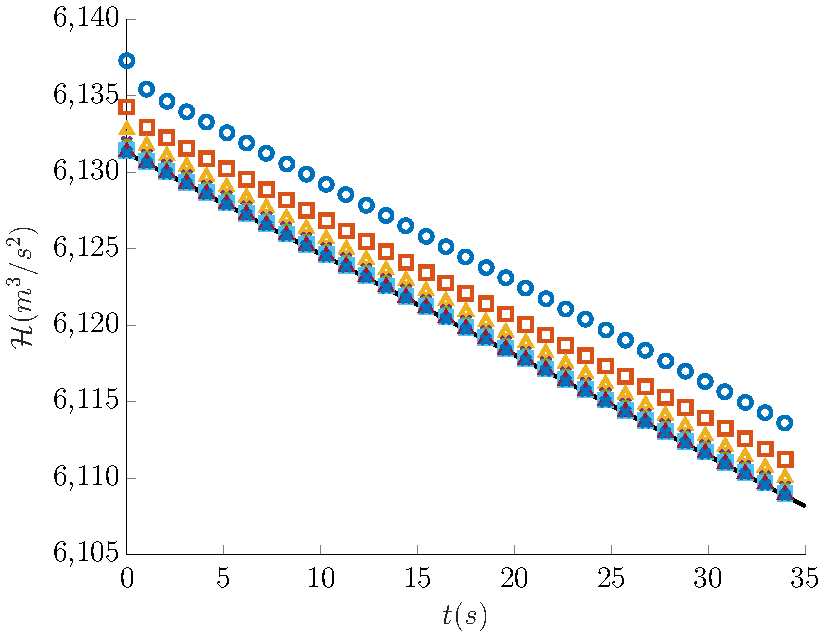
\includegraphics[width=0.6\textwidth]{./Figures/Simulations/Study/RegSWWE/Energy/EnergyOverTime.pdf}
	\caption{Energy over time for the numerical solutions, for the $\beta$ values in the Regularised SWWE family.}
\end{figure}


\subsection{Modified Dispersion Serre Family $\beta_2 = \beta_1$}
Justify interest, cite denys paper on dispersion modified equations

Points:
\begin{itemize}
	\item we do get nice well behaved transitions between behaviours when varying $\beta$
	\item Dispersive wave train location well approximated by using the linear wave speeds. Although the bump around these bounds suggests non-linear effects are important as well, particularly close to transitions across the wavespeed boundaries. 
	\item Improved dispersion may better approximate the dispsersion relation when $k\ll 1$, but at the cost of the middle of the dispersive wave train
	\item We get the bump behaviour observed in the db paper, but now dispersive wave trains are separate.
	\item Conservation is pretty similar, except for energy where it gets worse - this suggests that we will need finer grids to get good solutions particularly when gradients are large.
\end{itemize}

\begin{figure}
	\centering
	\begin{subfigure}{0.322\textwidth}
		\centering
		\includegraphics[width=\textwidth]{./Figures/Simulations/Study/ImpDisp/h.pdf}
		\caption{$h$}
	\end{subfigure}
	\begin{subfigure}{0.32\textwidth}
		\centering
		\includegraphics[width=\textwidth]{./Figures/Simulations/Study/ImpDisp/G.pdf}
		\caption{$G$}
	\end{subfigure}
	\begin{subfigure}{0.32\textwidth}
	\centering
	\includegraphics[width=\textwidth]{./Figures/Simulations/Study/ImpDisp/u.pdf}
	\caption{$u$}
	\end{subfigure}
	\caption{Plot of multiple smooth dambreak numerical solutions at $t=35s$.}
\end{figure}

\begin{figure}
	\centering
	\begin{subfigure}{0.32\textwidth}
		\centering
		\includegraphics[width=\textwidth]{./Figures/Simulations/Study/ImpDisp/hMiddle.pdf}
		\caption{$h$ in middle of dispersive wave train}
	\end{subfigure}
	\begin{subfigure}{0.32\textwidth}
		\centering
		\includegraphics[width=\textwidth]{./Figures/Simulations/Study/ImpDisp/GMiddle.pdf}
		\caption{$G$ in middle of dispersive wave train}
	\end{subfigure}
	\begin{subfigure}{0.32\textwidth}
	\centering
	\includegraphics[width=\textwidth]{./Figures/Simulations/Study/ImpDisp/uMiddle.pdf}
	\caption{$u$ in middle of dispersive wave train}
	\end{subfigure}
	\begin{subfigure}{0.32\textwidth}
	\centering
	\includegraphics[width=\textwidth]{./Figures/Simulations/Study/ImpDisp/hFront.pdf}
	\caption{$h$ Front of dispersive wave train}
	\end{subfigure}
	\begin{subfigure}{0.32\textwidth}
	\centering
	\includegraphics[width=\textwidth]{./Figures/Simulations/Study/ImpDisp/GFront.pdf}
	\caption{$G$ Front of dispersive wave train}
	\end{subfigure}
	\begin{subfigure}{0.32\textwidth}
	\centering
	\includegraphics[width=\textwidth]{./Figures/Simulations/Study/ImpDisp/uFront.pdf}
	\caption{$u$ Front of dispersive wave train}
	\end{subfigure}

	\caption{Plot of multiple smooth dambreak numerical solutions at important locations at $t=35s$.}
\end{figure}

\begin{figure}
	\centering
	\begin{subfigure}{0.49\textwidth}
		\centering
		\includegraphics[width=\textwidth]{./Figures/Simulations/Study/ImpDisp/Regions/hRegionsSerre.pdf}
		\caption{$\beta_1 = \beta_2 = 0$}
	\end{subfigure}
	\begin{subfigure}{0.49\textwidth}
		\centering
		\includegraphics[width=\textwidth]{./Figures/Simulations/Study/ImpDisp/Regions/hRegionsImpDisp.pdf}
		\caption{$\beta_1 = \beta_2 = \frac{1}{15}$}
	\end{subfigure}
	\caption{Regions of wave speeds for the smooth dambreak numerical solution at $t=35s$.}
\end{figure}



\begin{table}
	\centering
	\begin{tabular}{ c | c | c | c | c }
		$\beta_1$ & $h$ & $G$ & $uh$ & $\mathcal{H}$  \\
		\hline
		\T $0$ &	$8.0 \times 10^{-13}$ & $6.3 \times 10^{-13}$  & $3.3 \times 10^{-7}$ &	 $3.8 \times 10^{-6}$ \\
		\T$\dfrac{1}{30}$ & $8.1 \times 10^{-13}$ &	$6.4 \times 10^{-13}$ & $3.5 \times 10^{-7}$	 &	$1.9 \times 10^{-5}$ \\
		\T$\dfrac{1}{15}$ & $8.2 \times 10^{-13}$ &	$6.3 \times 10^{-13}$ & $5.8 \times 10^{-7}$	 &	$1.1 \times 10^{-4}$ \\
		
	\end{tabular}
	\caption{Conservation errors for Modified Dispersion Serre Equations for the solutions provided above with $\beta_2 = \beta_1 $.}
\end{table}



\subsection{Serre To SWWE Family $\beta_2 = 0$ and $-\frac{2}{3} \le \beta_1 \le 0$}
Justify interest, switching dispersion on and off, effect and giving structure/understanding to various schemes that turn it on and off.

Points:
\begin{itemize}
	\item we do get convergence, but most of the convergent behaviour occurs very close to the critical SWWE value. This is because gradients are large in the initial conditions
	\item Middle of dispersive wave train, and base and top of rarefaction fan most affected (closer to Serre)
	\item Still quite a large dispersive wave train even for $\beta_1$ values close to $-2/3$. (This appears to justify switching)
	\item the front of the shock became larger for some intermediate values.
	\item Trade-off between momentum convergence (since G = uh for SWWE) and energy convergence. Dispersive models conserve energy better due to smooth solutions, but conserve momentum worse because conserved quantitiy is not uh. 
\end{itemize}

\begin{figure}
	\centering
	\begin{subfigure}{0.32\textwidth}
		\centering
		\includegraphics[width=\textwidth]{./Figures/Simulations/Study/Serre2SWWECloser/h.pdf}
		\caption{$h$}
	\end{subfigure}
	\begin{subfigure}{0.32\textwidth}
		\centering
		\includegraphics[width=\textwidth]{./Figures/Simulations/Study/Serre2SWWECloser/G.pdf}
		\caption{$G$}
	\end{subfigure}
	\begin{subfigure}{0.32\textwidth}
	\centering
	\includegraphics[width=\textwidth]{./Figures/Simulations/Study/Serre2SWWECloser/u.pdf}
	\caption{$u$}
	\end{subfigure}
	\caption{Plot of multiple smooth dambreak numerical solutions at $t=35s$.}
\end{figure}



\begin{figure}
	\centering
	\begin{subfigure}{0.32\textwidth}
		\centering
		\includegraphics[width=\textwidth]{./Figures/Simulations/Study/Serre2SWWECloser/hMid.pdf}
		\caption{$h$ middle of dispersive wave train}
	\end{subfigure}
	\begin{subfigure}{0.32\textwidth}
		\centering
		\includegraphics[width=\textwidth]{./Figures/Simulations/Study/Serre2SWWECloser/GMid.pdf}
		\caption{$G$ middle of dispersive wave train}
	\end{subfigure}
	\begin{subfigure}{0.32\textwidth}
		\centering
		\includegraphics[width=\textwidth]{./Figures/Simulations/Study/Serre2SWWECloser/uMiddle.pdf}
		\caption{$u$ middle of dispersive wave train}
	\end{subfigure}
	\begin{subfigure}{0.32\textwidth}
	\centering
	\includegraphics[width=\textwidth]{./Figures/Simulations/Study/Serre2SWWECloser/hFront.pdf}
	\caption{$h$ front of dispersive wave train}
	\end{subfigure}
	\begin{subfigure}{0.32\textwidth}
		\centering
		\includegraphics[width=\textwidth]{./Figures/Simulations/Study/Serre2SWWECloser/GFront.pdf}
		\caption{$G$ front of dispersive wave train}
	\end{subfigure}
	\begin{subfigure}{0.32\textwidth}
		\centering
		\includegraphics[width=\textwidth]{./Figures/Simulations/Study/Serre2SWWECloser/uFront.pdf}
		\caption{$u$ front of dispersive wave train}
	\end{subfigure}
	\caption{Plot of multiple smooth dambreak numerical solutions at $t=35s$.}
\end{figure}


\begin{figure}
	\centering
	\begin{subfigure}{0.49\textwidth}
		\centering
		\includegraphics[width=\textwidth]{./Figures/Simulations/Study/Serre2SWWECloser/Regions/hRegionsSerre.pdf}
		\caption{$\beta_1 = \beta_2 = 0$}
	\end{subfigure}
	\begin{subfigure}{0.49\textwidth}
		\centering
		\includegraphics[width=\textwidth]{./Figures/Simulations/Study/Serre2SWWECloser/Regions/hRegionsSerreSWWEClose.pdf}
		\caption{$\beta_1 = -\frac{2}{3} + 10^{-3}$ and  $\beta_2 = 0$}
	\end{subfigure}
	\caption{Regions of wave speeds for the smooth dambreak numerical solution at $t=35s$.}
\end{figure}


\begin{table}
	\centering
	\begin{tabular}{ c | c | c | c | c }
		$\beta_1$ & $h$ & $G$ & $uh$ & $\mathcal{H}$  \\
		\hline
		\T $0$ &	$8.0 \times 10^{-13}$ &	$6.3 \times 10^{-13}$ & $3.3 \times 10^{-7}$ & $3.8 \times 10^{-6}$ \\
		\T $-\frac{2}{3} + 10^{-1}$ &	$7.2 \times 10^{-13}$ &	$6.3 \times 10^{-13}$ & $3.0 \times 10^{-6}$ & $6.3 \times 10^{-6}$ \\
		\T $-\frac{2}{3} + 10^{-2}$ &	$6.6 \times 10^{-13}$ &	$6.2 \times 10^{-13}$ & $3.2 \times 10^{-5}$ & $3.7 \times 10^{-4}$ \\		
		\T $-\frac{2}{3} + 10^{-3}$ &	$6.0 \times 10^{-13}$ &	$6.3 \times 10^{-13}$ & $1.2 \times 10^{-5}$ & $3.7 \times 10^{-3}$ \\	
		\T $-\frac{2}{3} + 10^{-4}$ &	$5.9 \times 10^{-13}$ &	$6.2 \times 10^{-13}$ & $1.2 \times 10^{-6}$ & $3.7 \times 10^{-3}$ 		
	\end{tabular}
	\caption{Conservation errors for Serre To SWWE Faimly of Equations for the solutions provided above with $\beta_2 = 0$ and $-\frac{2}{3}\le \beta_1 \le 0$.}
\end{table}




\end{document} 